% Options for packages loaded elsewhere
\PassOptionsToPackage{unicode}{hyperref}
\PassOptionsToPackage{hyphens}{url}
\documentclass[
]{article}
\usepackage{xcolor}
\usepackage[margin=1in]{geometry}
\usepackage{amsmath,amssymb}
\setcounter{secnumdepth}{-\maxdimen} % remove section numbering
\usepackage{iftex}
\ifPDFTeX
  \usepackage[T1]{fontenc}
  \usepackage[utf8]{inputenc}
  \usepackage{textcomp} % provide euro and other symbols
\else % if luatex or xetex
  \usepackage{unicode-math} % this also loads fontspec
  \defaultfontfeatures{Scale=MatchLowercase}
  \defaultfontfeatures[\rmfamily]{Ligatures=TeX,Scale=1}
\fi
\usepackage{lmodern}
\ifPDFTeX\else
  % xetex/luatex font selection
\fi
% Use upquote if available, for straight quotes in verbatim environments
\IfFileExists{upquote.sty}{\usepackage{upquote}}{}
\IfFileExists{microtype.sty}{% use microtype if available
  \usepackage[]{microtype}
  \UseMicrotypeSet[protrusion]{basicmath} % disable protrusion for tt fonts
}{}
\makeatletter
\@ifundefined{KOMAClassName}{% if non-KOMA class
  \IfFileExists{parskip.sty}{%
    \usepackage{parskip}
  }{% else
    \setlength{\parindent}{0pt}
    \setlength{\parskip}{6pt plus 2pt minus 1pt}}
}{% if KOMA class
  \KOMAoptions{parskip=half}}
\makeatother
\usepackage{color}
\usepackage{fancyvrb}
\newcommand{\VerbBar}{|}
\newcommand{\VERB}{\Verb[commandchars=\\\{\}]}
\DefineVerbatimEnvironment{Highlighting}{Verbatim}{commandchars=\\\{\}}
% Add ',fontsize=\small' for more characters per line
\usepackage{framed}
\definecolor{shadecolor}{RGB}{248,248,248}
\newenvironment{Shaded}{\begin{snugshade}}{\end{snugshade}}
\newcommand{\AlertTok}[1]{\textcolor[rgb]{0.94,0.16,0.16}{#1}}
\newcommand{\AnnotationTok}[1]{\textcolor[rgb]{0.56,0.35,0.01}{\textbf{\textit{#1}}}}
\newcommand{\AttributeTok}[1]{\textcolor[rgb]{0.13,0.29,0.53}{#1}}
\newcommand{\BaseNTok}[1]{\textcolor[rgb]{0.00,0.00,0.81}{#1}}
\newcommand{\BuiltInTok}[1]{#1}
\newcommand{\CharTok}[1]{\textcolor[rgb]{0.31,0.60,0.02}{#1}}
\newcommand{\CommentTok}[1]{\textcolor[rgb]{0.56,0.35,0.01}{\textit{#1}}}
\newcommand{\CommentVarTok}[1]{\textcolor[rgb]{0.56,0.35,0.01}{\textbf{\textit{#1}}}}
\newcommand{\ConstantTok}[1]{\textcolor[rgb]{0.56,0.35,0.01}{#1}}
\newcommand{\ControlFlowTok}[1]{\textcolor[rgb]{0.13,0.29,0.53}{\textbf{#1}}}
\newcommand{\DataTypeTok}[1]{\textcolor[rgb]{0.13,0.29,0.53}{#1}}
\newcommand{\DecValTok}[1]{\textcolor[rgb]{0.00,0.00,0.81}{#1}}
\newcommand{\DocumentationTok}[1]{\textcolor[rgb]{0.56,0.35,0.01}{\textbf{\textit{#1}}}}
\newcommand{\ErrorTok}[1]{\textcolor[rgb]{0.64,0.00,0.00}{\textbf{#1}}}
\newcommand{\ExtensionTok}[1]{#1}
\newcommand{\FloatTok}[1]{\textcolor[rgb]{0.00,0.00,0.81}{#1}}
\newcommand{\FunctionTok}[1]{\textcolor[rgb]{0.13,0.29,0.53}{\textbf{#1}}}
\newcommand{\ImportTok}[1]{#1}
\newcommand{\InformationTok}[1]{\textcolor[rgb]{0.56,0.35,0.01}{\textbf{\textit{#1}}}}
\newcommand{\KeywordTok}[1]{\textcolor[rgb]{0.13,0.29,0.53}{\textbf{#1}}}
\newcommand{\NormalTok}[1]{#1}
\newcommand{\OperatorTok}[1]{\textcolor[rgb]{0.81,0.36,0.00}{\textbf{#1}}}
\newcommand{\OtherTok}[1]{\textcolor[rgb]{0.56,0.35,0.01}{#1}}
\newcommand{\PreprocessorTok}[1]{\textcolor[rgb]{0.56,0.35,0.01}{\textit{#1}}}
\newcommand{\RegionMarkerTok}[1]{#1}
\newcommand{\SpecialCharTok}[1]{\textcolor[rgb]{0.81,0.36,0.00}{\textbf{#1}}}
\newcommand{\SpecialStringTok}[1]{\textcolor[rgb]{0.31,0.60,0.02}{#1}}
\newcommand{\StringTok}[1]{\textcolor[rgb]{0.31,0.60,0.02}{#1}}
\newcommand{\VariableTok}[1]{\textcolor[rgb]{0.00,0.00,0.00}{#1}}
\newcommand{\VerbatimStringTok}[1]{\textcolor[rgb]{0.31,0.60,0.02}{#1}}
\newcommand{\WarningTok}[1]{\textcolor[rgb]{0.56,0.35,0.01}{\textbf{\textit{#1}}}}
\usepackage{graphicx}
\makeatletter
\newsavebox\pandoc@box
\newcommand*\pandocbounded[1]{% scales image to fit in text height/width
  \sbox\pandoc@box{#1}%
  \Gscale@div\@tempa{\textheight}{\dimexpr\ht\pandoc@box+\dp\pandoc@box\relax}%
  \Gscale@div\@tempb{\linewidth}{\wd\pandoc@box}%
  \ifdim\@tempb\p@<\@tempa\p@\let\@tempa\@tempb\fi% select the smaller of both
  \ifdim\@tempa\p@<\p@\scalebox{\@tempa}{\usebox\pandoc@box}%
  \else\usebox{\pandoc@box}%
  \fi%
}
% Set default figure placement to htbp
\def\fps@figure{htbp}
\makeatother
\setlength{\emergencystretch}{3em} % prevent overfull lines
\providecommand{\tightlist}{%
  \setlength{\itemsep}{0pt}\setlength{\parskip}{0pt}}
\usepackage{bookmark}
\IfFileExists{xurl.sty}{\usepackage{xurl}}{} % add URL line breaks if available
\urlstyle{same}
\hypersetup{
  pdftitle={Effect of Education and Residence on Life Satisfaction -- WVS China 2018},
  pdfauthor={Alex Shen},
  hidelinks,
  pdfcreator={LaTeX via pandoc}}

\title{Effect of Education and Residence on Life Satisfaction -- WVS
China 2018}
\author{Alex Shen}
\date{2025-07-11}

\begin{document}
\maketitle

\subsection{Data and Methods}\label{data-and-methods}

World Values Survey, Wave 7 (China, 2018). Logistic regression
predicting high life satisfaction (score ≥ 7) by education, urban/rural
status, age, and sex, with education × urban interaction.

\begin{Shaded}
\begin{Highlighting}[]
\CommentTok{\# Adjust the path as needed}
\NormalTok{df\_raw }\OtherTok{\textless{}{-}} \FunctionTok{read\_excel}\NormalTok{(}\StringTok{"data/F00013183{-}WVS\_Wave\_7\_China\_Excel\_v5.1.xlsx"}\NormalTok{, }\AttributeTok{sheet =} \DecValTok{1}\NormalTok{)}
\NormalTok{df }\OtherTok{\textless{}{-}}\NormalTok{ df\_raw }\SpecialCharTok{\%\textgreater{}\%}
  \FunctionTok{transmute}\NormalTok{(}
    \AttributeTok{life\_satisfaction =} \FunctionTok{as.numeric}\NormalTok{(}\StringTok{\textasciigrave{}}\AttributeTok{Q49: Satisfaction with your life}\StringTok{\textasciigrave{}}\NormalTok{),}
    \AttributeTok{education =} \FunctionTok{factor}\NormalTok{(}
      \FunctionTok{as.numeric}\NormalTok{(}\StringTok{\textasciigrave{}}\AttributeTok{Q275R: Highest educational level: Respondent (recoded into 3 groups)}\StringTok{\textasciigrave{}}\NormalTok{),}
      \AttributeTok{levels =} \DecValTok{1}\SpecialCharTok{:}\DecValTok{3}\NormalTok{,}
      \AttributeTok{labels =} \FunctionTok{c}\NormalTok{(}\StringTok{"Primary"}\NormalTok{, }\StringTok{"Secondary"}\NormalTok{, }\StringTok{"Tertiary"}\NormalTok{)}
\NormalTok{    ),}
    \AttributeTok{urban =} \FunctionTok{as.numeric}\NormalTok{(}\StringTok{\textasciigrave{}}\AttributeTok{H\_URBRURAL: Urban{-}Rural}\StringTok{\textasciigrave{}}\NormalTok{),}
    \AttributeTok{age =} \FunctionTok{as.numeric}\NormalTok{(}\StringTok{\textasciigrave{}}\AttributeTok{Q262: Age}\StringTok{\textasciigrave{}}\NormalTok{),}
    \AttributeTok{sex =} \FunctionTok{as.numeric}\NormalTok{(}\StringTok{\textasciigrave{}}\AttributeTok{Q260: Sex}\StringTok{\textasciigrave{}}\NormalTok{)}
\NormalTok{  ) }\SpecialCharTok{\%\textgreater{}\%}
  \FunctionTok{filter}\NormalTok{(}
    \SpecialCharTok{!}\FunctionTok{is.na}\NormalTok{(life\_satisfaction), }\SpecialCharTok{!}\FunctionTok{is.na}\NormalTok{(education), }\SpecialCharTok{!}\FunctionTok{is.na}\NormalTok{(urban), }\SpecialCharTok{!}\FunctionTok{is.na}\NormalTok{(age), }\SpecialCharTok{!}\FunctionTok{is.na}\NormalTok{(sex)}
\NormalTok{  ) }\SpecialCharTok{\%\textgreater{}\%}
  \FunctionTok{mutate}\NormalTok{(}
    \AttributeTok{urban\_bin =} \FunctionTok{if\_else}\NormalTok{(urban }\SpecialCharTok{==} \DecValTok{1}\NormalTok{, }\DecValTok{1}\NormalTok{, }\DecValTok{0}\NormalTok{),}
    \AttributeTok{satisfied =} \FunctionTok{if\_else}\NormalTok{(life\_satisfaction }\SpecialCharTok{\textgreater{}=} \DecValTok{7}\NormalTok{, }\DecValTok{1}\NormalTok{, }\DecValTok{0}\NormalTok{)}
\NormalTok{  )}
\FunctionTok{nrow}\NormalTok{(df)}
\end{Highlighting}
\end{Shaded}

\begin{verbatim}
## [1] 3006
\end{verbatim}

\begin{Shaded}
\begin{Highlighting}[]
\NormalTok{model }\OtherTok{\textless{}{-}} \FunctionTok{glm}\NormalTok{(satisfied }\SpecialCharTok{\textasciitilde{}}\NormalTok{ education }\SpecialCharTok{*}\NormalTok{ urban\_bin }\SpecialCharTok{+}\NormalTok{ age }\SpecialCharTok{+}\NormalTok{ sex, }\AttributeTok{data =}\NormalTok{ df, }\AttributeTok{family =} \StringTok{"binomial"}\NormalTok{)}
\FunctionTok{summary}\NormalTok{(model)}
\end{Highlighting}
\end{Shaded}

\begin{verbatim}
## 
## Call:
## glm(formula = satisfied ~ education * urban_bin + age + sex, 
##     family = "binomial", data = df)
## 
## Coefficients:
##                               Estimate Std. Error z value Pr(>|z|)    
## (Intercept)                  -0.135423   0.222617  -0.608   0.5430    
## educationSecondary            0.295802   0.188457   1.570   0.1165    
## educationTertiary             0.496872   0.250355   1.985   0.0472 *  
## urban_bin                    -0.022624   0.108451  -0.209   0.8347    
## age                           0.017344   0.003169   5.473 4.43e-08 ***
## sex                           0.087271   0.081581   1.070   0.2847    
## educationSecondary:urban_bin -0.122208   0.222885  -0.548   0.5835    
## educationTertiary:urban_bin  -0.076170   0.271535  -0.281   0.7791    
## ---
## Signif. codes:  0 '***' 0.001 '**' 0.01 '*' 0.05 '.' 0.1 ' ' 1
## 
## (Dispersion parameter for binomial family taken to be 1)
## 
##     Null deviance: 3624.2  on 3005  degrees of freedom
## Residual deviance: 3591.3  on 2998  degrees of freedom
## AIC: 3607.3
## 
## Number of Fisher Scoring iterations: 4
\end{verbatim}

\begin{Shaded}
\begin{Highlighting}[]
\NormalTok{df }\SpecialCharTok{\%\textgreater{}\%}
  \FunctionTok{group\_by}\NormalTok{(education, urban\_bin) }\SpecialCharTok{\%\textgreater{}\%}
  \FunctionTok{summarise}\NormalTok{(}\AttributeTok{mean\_satisfied =} \FunctionTok{mean}\NormalTok{(satisfied, }\AttributeTok{na.rm =} \ConstantTok{TRUE}\NormalTok{)) }\SpecialCharTok{\%\textgreater{}\%}
  \FunctionTok{ggplot}\NormalTok{(}\FunctionTok{aes}\NormalTok{(}\AttributeTok{x =}\NormalTok{ education, }\AttributeTok{y =}\NormalTok{ mean\_satisfied, }\AttributeTok{fill =} \FunctionTok{factor}\NormalTok{(urban\_bin, }\AttributeTok{labels =} \FunctionTok{c}\NormalTok{(}\StringTok{"Rural"}\NormalTok{, }\StringTok{"Urban"}\NormalTok{)))) }\SpecialCharTok{+}
  \FunctionTok{geom\_bar}\NormalTok{(}\AttributeTok{stat =} \StringTok{"identity"}\NormalTok{, }\AttributeTok{position =} \StringTok{"dodge"}\NormalTok{) }\SpecialCharTok{+}
  \FunctionTok{labs}\NormalTok{(}
    \AttributeTok{x =} \StringTok{"Education Level"}\NormalTok{,}
    \AttributeTok{y =} \StringTok{"Proportion Satisfied"}\NormalTok{,}
    \AttributeTok{fill =} \StringTok{"Residence"}\NormalTok{,}
    \AttributeTok{title =} \StringTok{"Effect of Education and Residence on Life Satisfaction"}
\NormalTok{  ) }\SpecialCharTok{+}
  \FunctionTok{theme\_minimal}\NormalTok{()}
\end{Highlighting}
\end{Shaded}

\pandocbounded{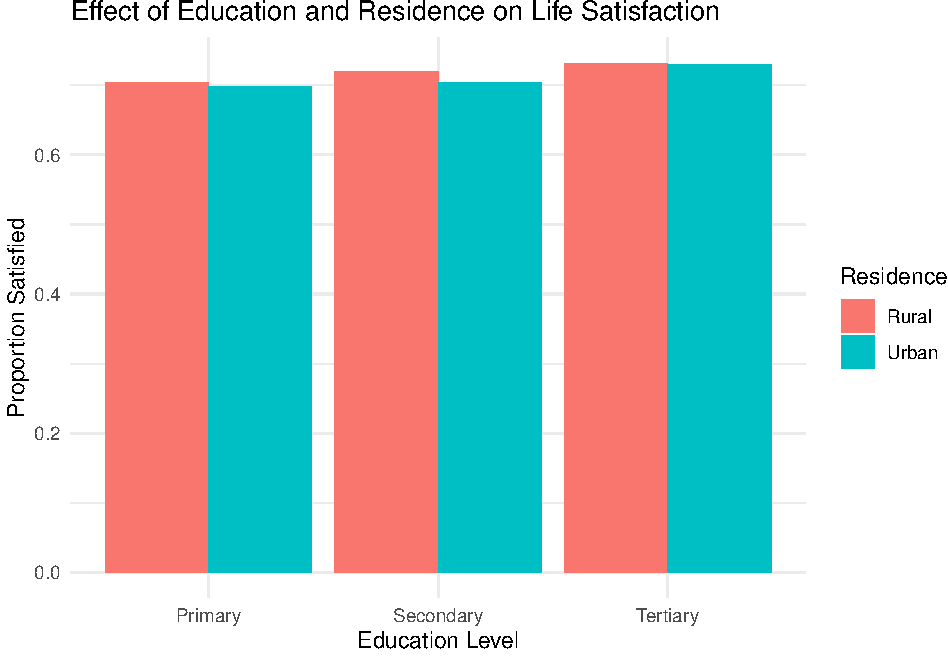
\includegraphics[keepaspectratio]{urban_educ_happiness_files/figure-latex/visualization-1.pdf}}

\end{document}
